Таким образом, решено было использовать эвристические алгоритмы оптимизации:
\href{https://en.wikipedia.org/wiki/Simulated_annealing}{Генетический алгоритм} и \href{https://en.wikipedia.org/wiki/Simulated_annealing}{Симуляция отжига}.

\subsection{Представление «решения»  — набора мазков}
Программа работает с последовательностями мазков, находя лучшую из них.
Однако, чтобы алгоритм оптимизации работал с ними, наборы мазков должны быть представлены в виде векторов в $\mathbb{R}^n$.
Формат данных в «геноме» таков:

\begin{figure}[h]
    \centering
    \adjincludegraphics[width=0.7\textwidth, clip, trim={0.15\width} {0.7\height} {0.15\width} {0.125\height}]{genome_contents_table.pdf}
    \caption{Схема хранения генома}
    \label{fig:genome_contents_table}
\end{figure}


, где $p_{n_x} ~\&\&~ p_{n_y}, n \in \{ 0, 1, 2 \}$ — координаты направляющей точки под номером n (из всего 3 у каждого мазка),
а \textit{width}  — толщина мазка.

Здесь нет параметра  «цвет».
Причина объяснена в разделе: \ref{subsec:color_in_genome}.

\subsection{Задание функции ошибки}
Чтобы решить задачу алгоритмом оптимизации, нужна некая метрика — функция, которая будет определять степень «неподходящести» данного ей решения.
Именно она будет передаваться алгоритму оптимизации.
В нашем случае вычисление ФО включает в себя растеризацию мазков (отображение их на изображении) и вычисления, производящие сравнения полученного результата с желаемым.
Функцию ошибки необходимо задать таким образом, чтобы она отражала качество полученной комбинации мазков,
причём в любой точке направление её уменьшения соответствовало направлению улучшения результата.
Помимо напрашивающегося \href{https://en.wikipedia.org/wiki/Mean_squared_error}{MSE}

\begin{equation}\label{eq:equation}
    MSE = \sum_{y = 0}^{y < height} { \sum_{x = 0}^{x < width} { \sum_{c \in  \left\{ r, g, b \right\} } { \left( {\overrightarrow {rendered_{x, y}}}_c - {\overrightarrow{original_{x, y}}}_c\right)^2 }}}
\end{equation}

, повсеместно используемого при работе с изображениями, функция ошибки «наказывает» наложение мазков, а также


\subsection{Растеризация мазков}\label{subsec:rasterization}
Имея мазок, заданный в виде трёх точек на плоскости, толщины и цвета, нужно уметь его отобразить его на «холсте», то есть в виде набора пикселей.
Это нужно, чтобы подсчитать функцию ошибки для заданного набора мазков,
причём так, чтобы результат максимально соответствовал мазку, рисуемому роботом.
В качестве достаточно точной модели описания такого мазка возьмём круглую кисть, перемещающуюся по заданной траектории.
Есть много способов произвести растеризацию.
Нужно выбрать тот, который будет производительным и в то же время максимально близким к реальному мазку.

Самый простой — для некоторого количества точек на кривой Безье (с достаточно маленьким шагом, примерно один пиксель) проводим вертикальную линию: вверх на width и  вниз — тоже.
Это даёт высокую производительность и сносно выглядит на участках, близких к горизонтальным, но результат, полученный таким способом, очень далёк от реальности на вертикальных участках:
\begin{figure}[h!]
    \centering
    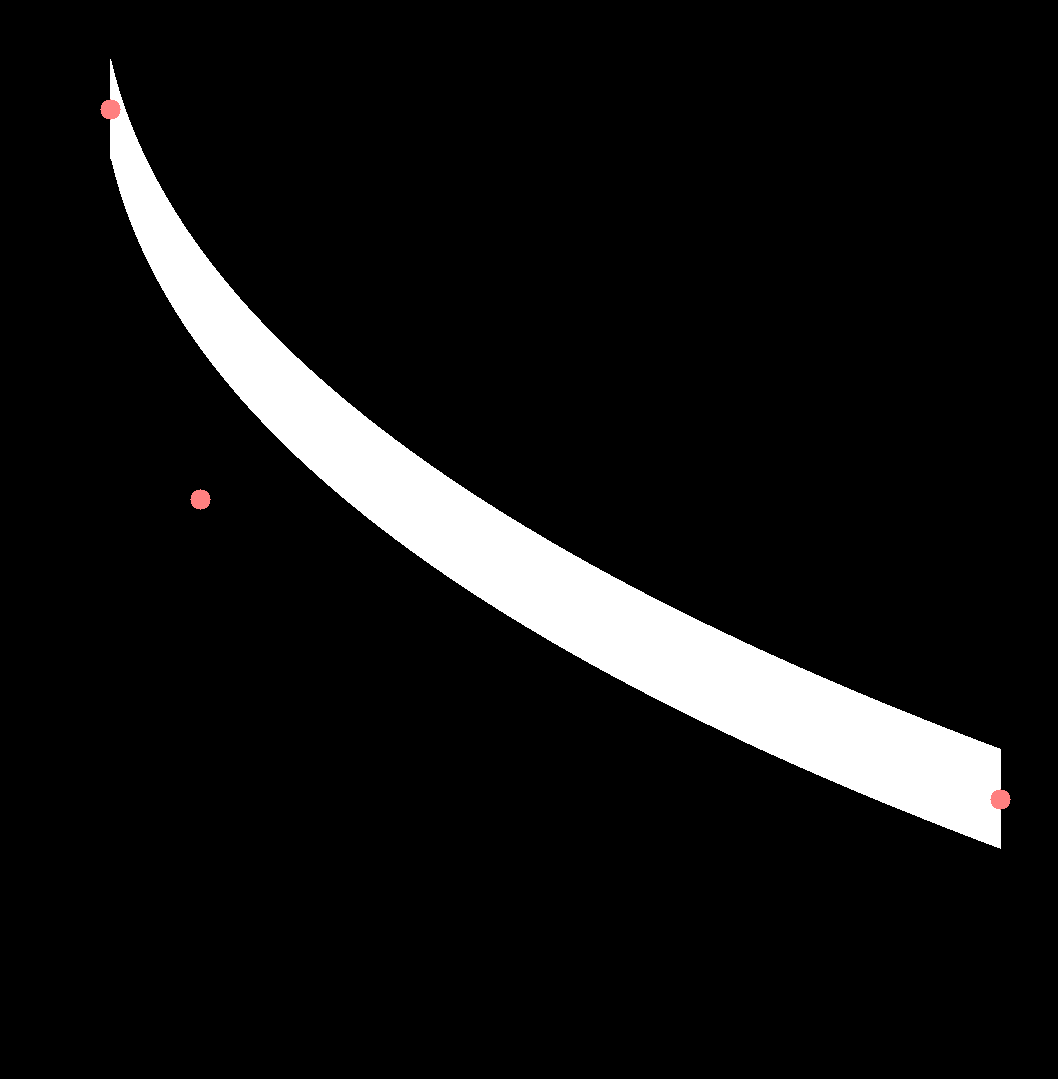
\includegraphics[width=0.75\textwidth]{stroke_vertical.png}
    \caption{(Красным обозначены точки, задающие кривую)}
    \label{fig:vertical_stroke}
\end{figure}
\begin{figure}
    \centering
    
\includegraphics[width=0.75\textwidth]{one_stroke.png}
    \caption{Иногда такой способ добавляет свой шарм}
    \label{fig:pretty_vert_stroke}
\end{figure}

Есть разные способы избавиться от этих недостатков, сохраняя максимальную производительность.
Например:
\begin{itemize}
    \item Совмещать горизонтальные и вертикальные полосы
    \item Проводить полосы перпендикулярно направлению кривой в данной точке
\end{itemize}
В каждом из них будут наблюдаться пустые места, полости, что недопустимо.

Ультимативным же способом является подражание реальной жизни: «проведение» круглой «кистью» по экрану.
То есть берутся точки на кривой на небольшом расстоянии друг от друга, и с центром в каждой из них рисуется круг радиусом width.
Однако в таком случае каждая точка, попадающая в мазок обрабатывается много раз (для близких кругов), что значительно замедляет рендерниг.
Если же увеличить шаг, этой проблемы можно частично избежать, но мазок стал бы неровным.
При маленьком шаге это выглядит так:
\begin{figure}[h!]
    \centering
    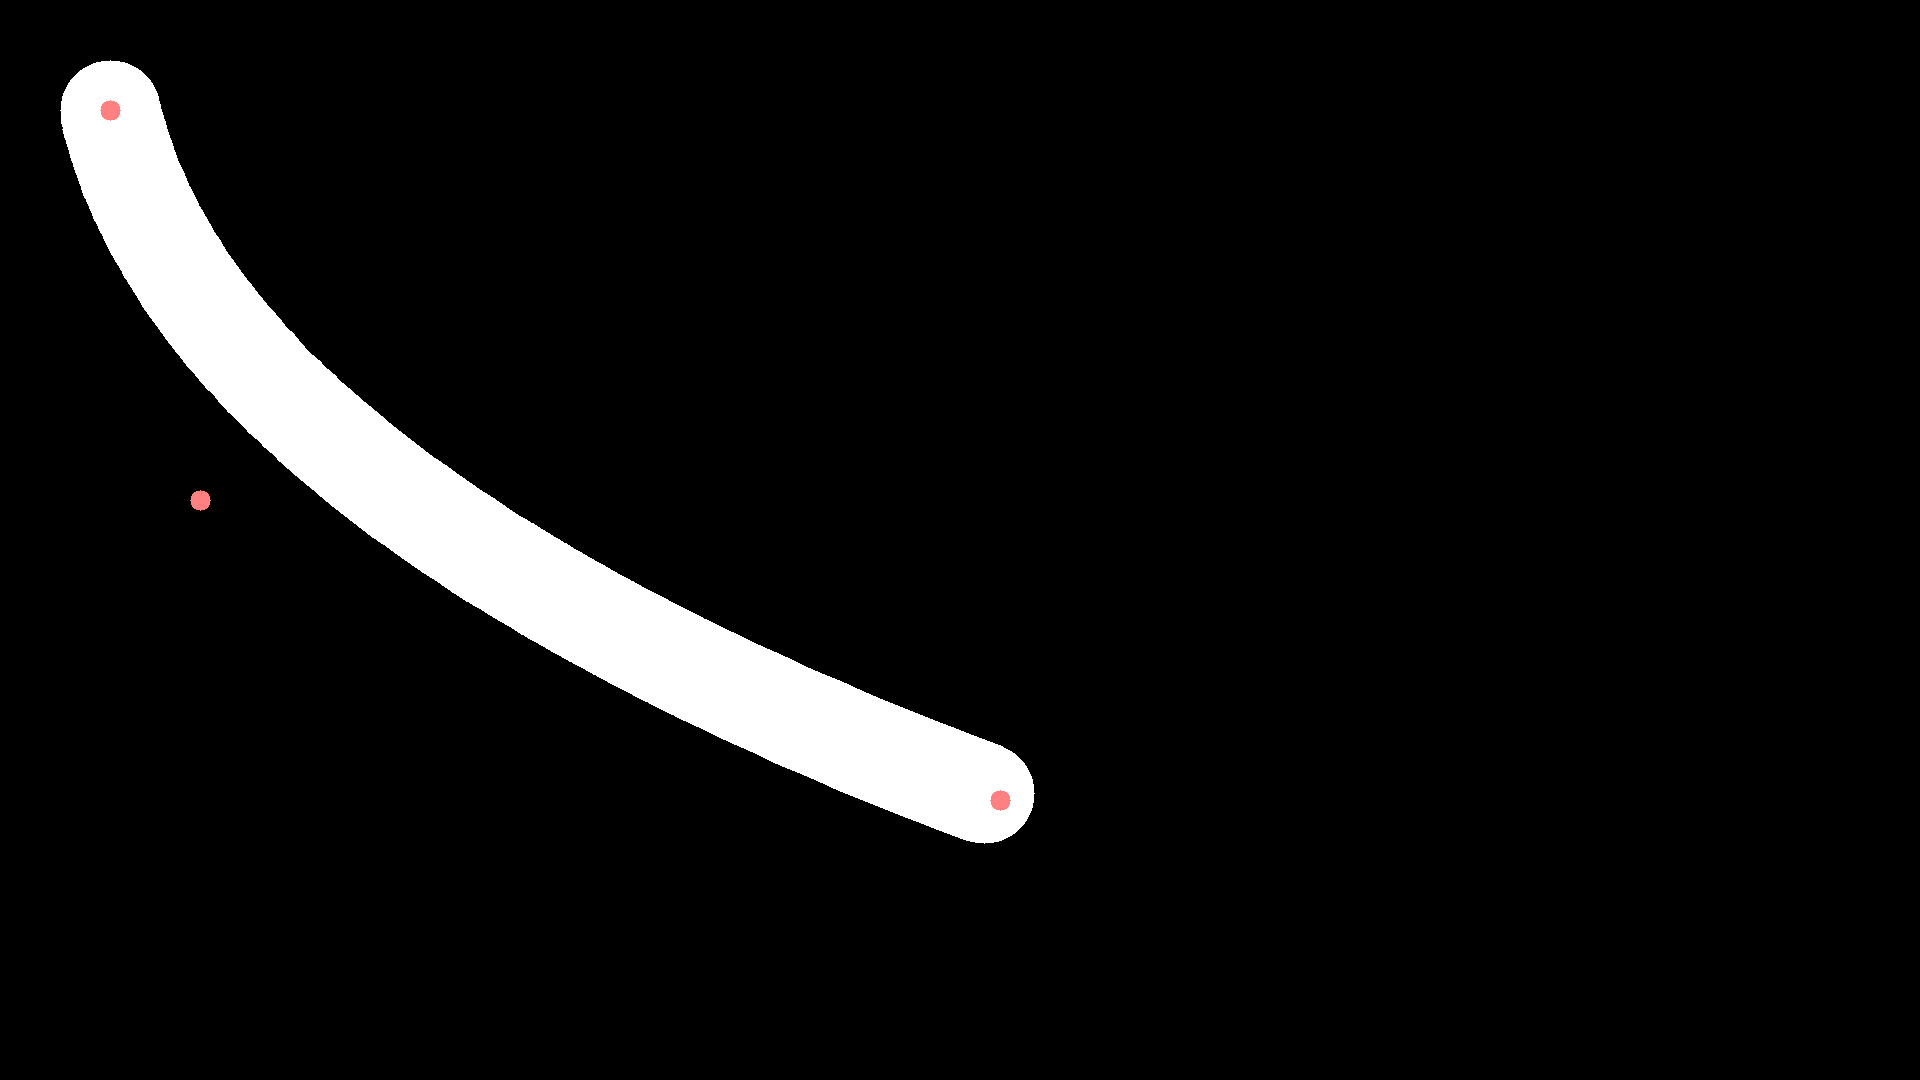
\includegraphics[width=0.75\textwidth]{stroke_smooth.png}
    \label{fig:smooth_stroke}
\end{figure}

В будущем планируется улучшить алгоритм для ускорения растеризации при почти том же качестве.
Рассматриваются варианты:
\begin{itemize}
    \item Заменить круглую кисть на также гладкую, но с более медленным закруглением с дальней от вектора кривой в данной точке стороны, поворачивая кисть соответствующим образом:
    \begin{figure}
        \centering
        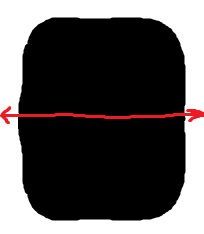
\includegraphics[width=0.75\textwidth]{modern_brush.png}
        \caption{(красным обозначено направление вектора кривой)}
        \label{fig:modern_brush}
    \end{figure}
    Такое изменение поможет уменьшить артефакты при увеличении шага между точками на кривой, то есть позволит сделать шаг больше, ускорив процесс.

    \item Автоматически разбивать мазок на «полигоны».
                Для этого нужно пройтись по кривой и с некоторым шагом (уже побольше, чем раньше),
                отметить для каждой рассматриваемой точки на прямой, содержащей её и перпендикулярной текущему направлению, точки в обе стороны от неё на расстоянии width.
                Каждая из них добавляется в соответствующий стороне в порядке обхода список.
                Потом полигоны, полученные из соседних точек на кривой и соответствующим им вынесенным точкам, заливаются нужным цветом.
                На концах же мазка рендерятся круги.

    \begin{figure}
        \centering
        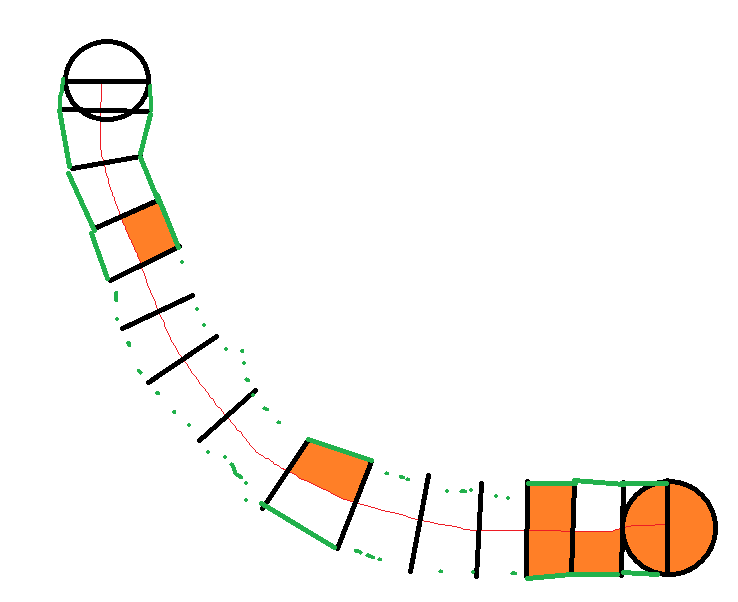
\includegraphics[width=0.75\textwidth]{polygonal_stroke.png}
        \caption{Схема полигональной разбивки мазка}
        \label{fig:polygonal_stroke}
    \end{figure}

    При использовании этого метода никакая существенная часть пикселей мазка не обрабатывается по много раз, что говорит о высокой эффективности алгоритма.
    Поэтому я собираюсь внедрить такой метод в ближайшее время.
\end{itemize}

Что же касается совместимости с видеокартой,
для круга и модифицированной кисти понятно, как определить bouding-box,
и понятно, как по координатам пикселя быстро определить, принадлежит ли он этому примитиву.
А рендеринг полигонов производится аппаратно.

Подробнее про внедрение видеокарты можно почитать в разделе \ref{subsec:move_graphics_to_videocard}.

\subsection{Учёт цвета при оптимизации}\label{subsec:color_in_genome}
Как происходит пастеризация, работа с зонами: \ref{subsec:posterisation_and_zoning}